%%%%%%%%%%%%%%%%%%%%%%%%%%%%%%%%%%%%%%%%%%%%%%%%%%%%%%%%%%%%%%%%%%%%%%%%%%%%%%%
%%                                                                   CERN & LHC
%%%%%%%%%%%%%%%%%%%%%%%%%%%%%%%%%%%%%%%%%%%%%%%%%%%%%%%%%%%%%%%%%%%%%%%%%%%%%%%
%%                                             Few words about CERN and the LHC

\chapter{Experimenteller Aufbau}
\label{experimenteller_aufbau}

\begin{quote}
    The abstract comes last
\end{quote}

%______________________________________________________________________________
%                                                                    CERN & LHC
%
\section{Der Large Hadron Collider}
\label{lhc}

Der \acf{LHC} ist der derzeit leistungsstärkste Teilchenbeschleuniger der Welt
und steht am CERN\footnote{\acf{CERN}} nahe Genf in der Schweiz. Die
Fertigstellung erfolgte 2008 unter Beiteiligung von über einhundert Nationen.
Der \ac{LHC} ist ein Hadronen-Speicherring mit knapp $27\;\kilo\meter$ Umfang,
der in den Tunnel des Vorgänger-Beschleunigers LEP\footnote{\acf{LEP}} zwischen
50m und 100m unter der Erdoberfläche, gebaut wurde. Im Kern ist der
\ac{LHC} ein Synchrotron, dass Protonen oder Blei-Ionen in gegenläufigen
Teilchenstrahlen auf annähernd Lichtgeschwindigkeit beschleunigt und an
fest-definierten Punkten zur Kollision bringt. Zuvor durchlaufen die Teilchen
einige Vorbeschleunigerstufen, die bereits eine Energie von $900\GeV$ zur
Verfügung stellen.  Die Kollisionspunkte der Teilchenstrahlen liegen innerhalb
der Detektoren der Experimente. Die vier größten Experimente sind \acs{ATLAS},
CMS, ALICE und LHCb, deren Lage in Abbildung \ref{fig:LHC} zu sehen ist.

\begin{figure}[h]
    \centering
    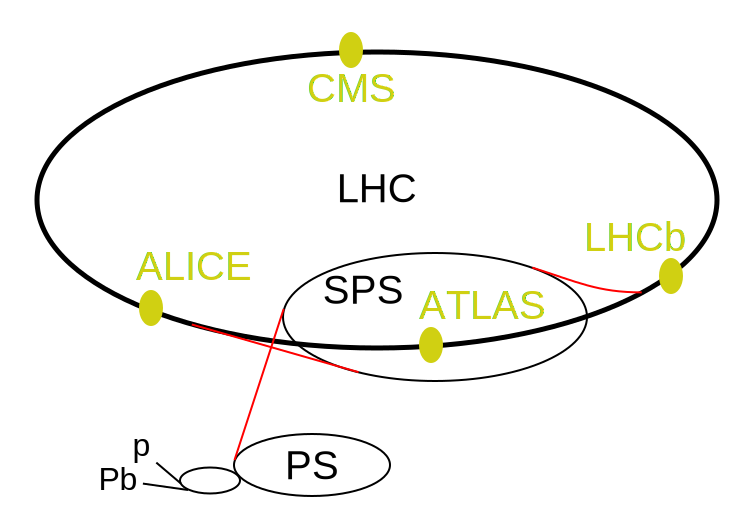
\includegraphics[width=0.5\textwidth]{img/LHC}
    \caption[Zeichnung des LHC mit Vorbeschleunigern und Experimenten]
        {Schematische Zeichnung des LHC mit den vier größten Experimenten und
        den letzten Vorbeschleunigerstufen (PS, SPS)}
    \label{fig:LHC}
\end{figure}

Der \ac{LHC} wird prinzipiell in zwei Modi betrieben: Proton-Proton Kollisionen
oder Proton-Blei Kollisionen. Aufgrund der Relevanz für die vorliegende Arbeit
wird im Folgenden auschließlich auf erstgenannte eingegangen. In Proton-Proton
Kollisionen erreichte der \ac{LHC} zuletzt Schwerpunktsenergien von $8\TeV$ und
befindet sich zum Zeitpunkt dieser Arbeit in der ersten großen Wartungsphase
nach deren Abschluss die Design-Schwerpunktsenergie von $14\TeV$ erreicht
werden soll.

Die Teilchen werden in Paketen, sog. \textit{Bunches} (vom engl. \textit{bunch}
- Bündel) von je etwa $10^{11}$ Teilchen in den \ac{LHC} eingespeist, welche
mit einer Rate von $40\mega\hertz$ in den Teilchendetektoren kollidieren.
Zuvor werden die Pakete durch Magnete auf die Kollisionspunkte fokusiert, um
deren Querschnittsfläche zu minimieren und somit die Luminosität zu maximieren
(siehe Gleichung \ref{eq:collider_lumi}). So konnten bisher Luminositäten von
bis zu $8\cdot 10^{-33} \centi\meter^{-2}\second^{-1}$ gemessen werden.



%______________________________________________________________________________
%                                                            Der ATLAS Detektor
%
\section{Der ATLAS Detektor}
\label{atlas_detector}

% + Skimms und Slimms, D3PD (auch Verweis auf DAQ)
% + GRL, Fills/Runs, LumiBlocks

Der ATLAS Detektor\footnote{\acf{ATLAS}} ist ein Vielzweck Teilchendetektor und
eines der vier Hauptexperimente am \ac{LHC}. Mit $44\meter$ Länge, $25\meter$
Durchmesser und etwa $7000\ton$ Gewicht ist es zugleich auch das größte der
Experimente. Der grundlegende Aufbau gleicht einem Schalenmodell und ist
symmetrisch um die Strahlachse angelegt (siehe Abbildung \ref{fig:atlas}).

\begin{figure}
    \centering
    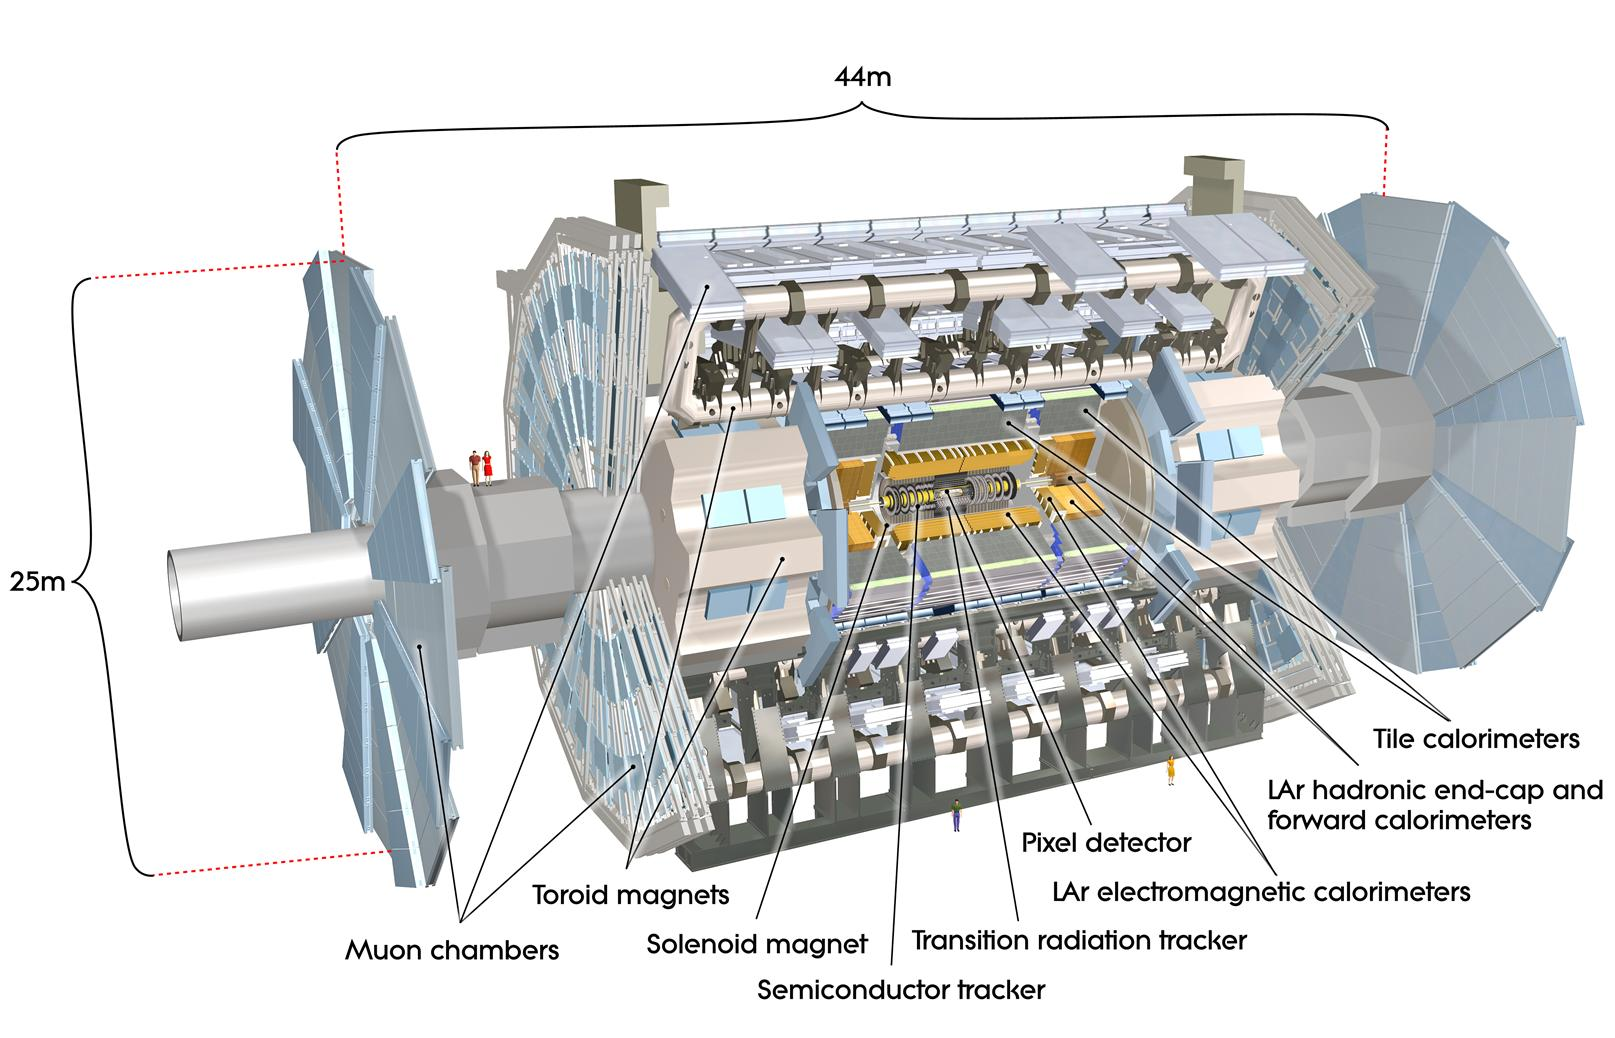
\includegraphics[width=1.0\textwidth]{img/atlas}
    \caption[Aufgeschnittene Darstellung des ATLAS Detektors]
        {Aufgeschnittene Darstellung des ATLAS Detektors}
    \label{fig:atlas}
\end{figure}

Dabei befindet sich unmittelbar um die Strahlachse der innere Detektor zur
Bestimmung der Vertexposition und zur Spurmessung. In diesem Bereich herrscht
ein solenoides Magentfeld von etwa $2\tesla$ stärke. Den inneren Detektor
umgebend schließen sich das elektromagnetische und das hadronische Kalorimeter
zur Messung der Energie an. Die äußerste Schale stellt das Myon-System dar,
welches von einem toroidalen Magentfeld durchzogen wird.

Bevor die einzelnen Komponenten näher erläutert werden ist es zweckmäßig das in
ATLAS verwendet Koordinatensystem zu definieren. Ausgangspunkt hierfür ist der
nominelle Wechselwirkungspunkt im Zentrum des Detektors, welcher den Nullpunkt
darstellt. Die Strahlachse und zugleich radiale Symmetrieachse des Detektors
wird als z-Achse festgelegt. Die x-Achse zeigt orthogonal zur Strahlachse auf
die Mitte des Beschleuniger-Rings, während die y-Achse noch oben zeigt und
somit ein Rechtssystem entsteht. Aufgrund der symmetrischen Geometrie des
Detektors definiert man nun für Richtungsangaben einen Azimuthwinkel
$\phi$ in der x-y-Ebene um die Strahlachse, wobei die positive x-Achse der
Ebene mit $\phi=0$ entspricht, und die Pseudorapidität $\eta$ anstelle des
Polarwinkels $\theta$:
\begin{equation}
    \eta \; = \; - \ln \left( \tan\frac{\theta}{2} \right)
\end{equation}
Die Verwendung der Pseudorapidität ist gebräuchlich, da die Rate der in
Proton-Kollisionen erzeugten Teilchen als Funktion von $\eta$ annähernd
konstant ist. Abstände in der $\eta$-$\phi$ Ebene werden mit
$R=\sqrt{\eta^2-\phi^2}$ angegeben.

Im Folgenden werden nun die zum Nachweis von Elektronen relevanten Komponenten
des Detektors und deren Funktionsweise näher erläutert.



\subsection{Innerer Detektor}
\label{inner_detector}

Der innere Detektor bildet das Spurerkennungssystem von ATLAS und besteht im
wesentlichen aus drei Hauptkomponenten. Von innen nach außen folgen der
Pixeldetektor, der \acf{SCT} und der \acf{TRT}. Abbildung
\ref{fig:inner_detector} zeigt den Aufbau des inneren Detektors. Die Aufgabe
des inneren Detektor ist die Rekonstruktion der spuren geladener Teilchen,
woraus die Position des Wechselwirkungs-Vertex bestimmt wird. Desweiteren wird
aus der durch das anliegende solenoide Magnetfeld induzierten Krümmung der
Teilchenspuren deren transversaler Impuls\footnote{transversaler Impuls meint
die Impulskomponente senkrecht zur Strahlachse (z-Achse)} bestimmt. Ebenso
lässt sich auch die Ladung eines Teilchens aus der Krümmung bestimmen.

\begin{figure}
    \centering
    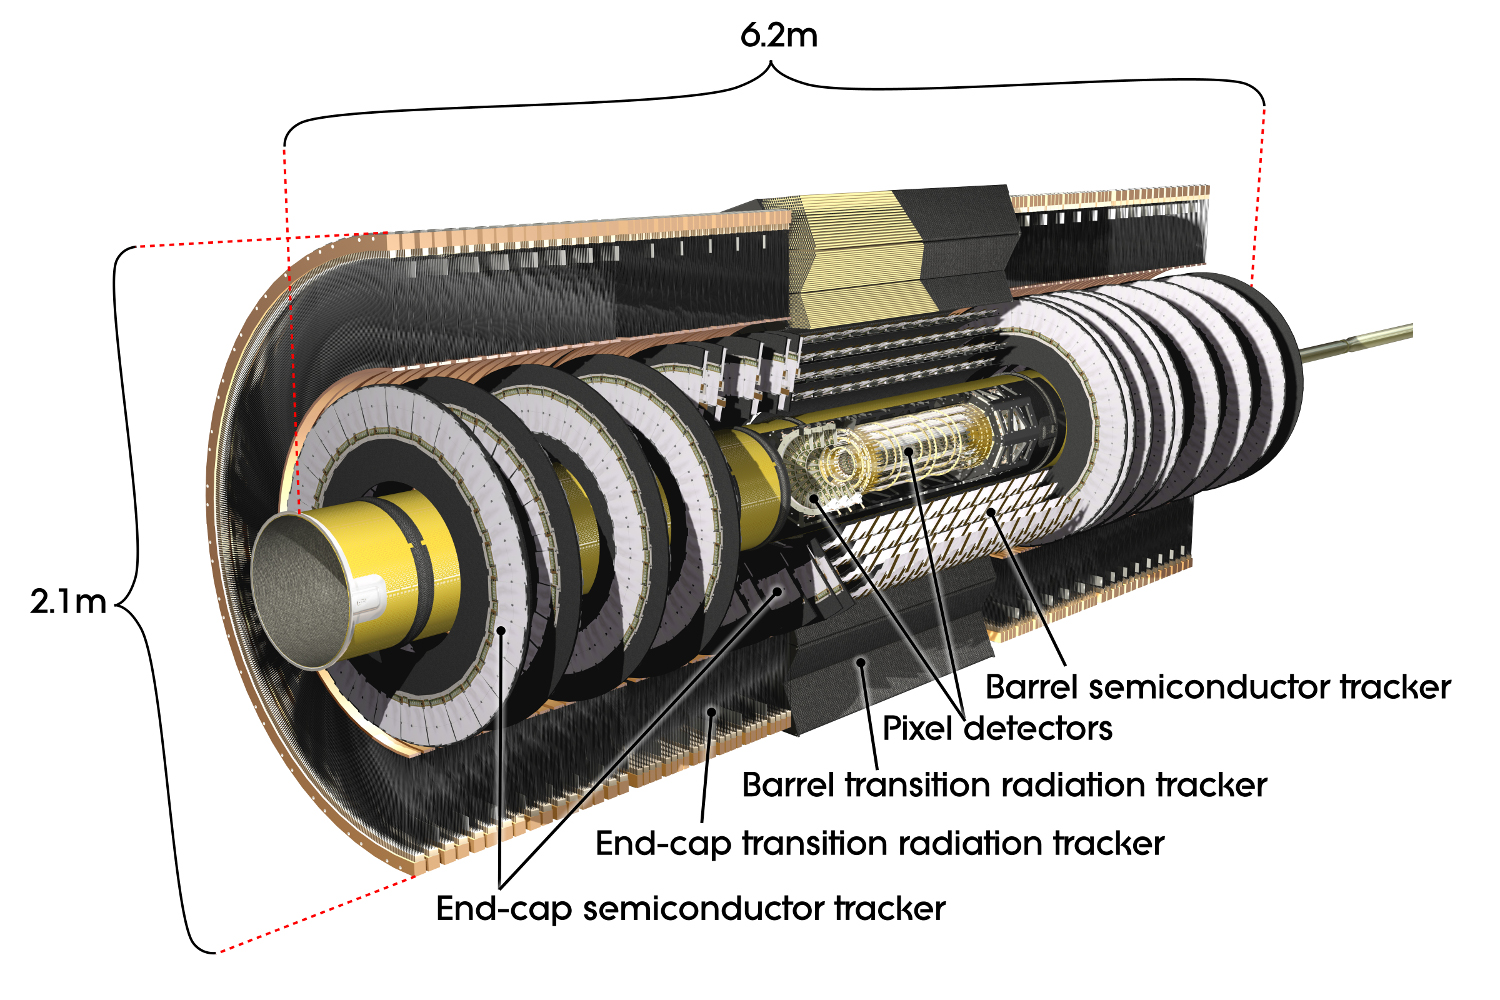
\includegraphics[width=.8\textwidth]{img/inner_detector}
    \caption[Darstellung des inneren Detektors]
        {Aufgeschnittene Darstellung des inneren Detektors}
    \label{fig:inner_detector}
\end{figure}

Der Pixeldetektor besteht aus drei zylindrisch angelegten Lagen von
Silzium-Pixeln im Zentrum, sowie je drei weiteren scheibenförmigen Lagen
konzentrisch angedordnet links und rechts davon. Insgesamt wird so ein Bereich
von $|\eta| < 2.5$ abgedeckt. Die erste zylindrische Lage hat dabei einen
Abstand von gerademal $45\milli\meter$ zur Strahlachse. Die Aufgabe des
Pixeldetektors ist räumliche Auflösung der Teilchenspuren zur Bestimmung des
Primärvertex, also der Position der ursprünglichen Wechselwirkung. Zudem lassen
sich Sekundärvertizes nahe an der Strahlachse erkennen, die Entstehen, wenn
Teilchen sich als Zwischenprodukte vom Primärvertex entfernen und erst abseits
zerfallen. Da ein solches Verhalten typisch für b-Quarks ist, wird die erste
der drei Pixel-Lagen auch \textit{b-layer} (vom engl. \textit{layer}, Lage)
genannt. Der Pixeldetektor erlaubt eine räumliche Auflösung von
$10\micro\meter$ in der $R$-$\phi$ Ebene und $115\micro\meter$ in z-Richtung.

Die nächste Schale bildet der \acf{SCT}, der mit einer Abdeckung von ebenfalls
$|\eta| < 2.5$ aus vier zylindrischen Lagen im Zentrum und neun Lagen auf jeder
Seite in Scheibenform. Auch hier kommen Halbleiter-Detektoren zum Einsatz, die
hier allerdings in Streifenform konstruiert wurden. Da mit größerem Radius die
Dichte der nachzuweisenden Spuren abnimmt ist hier eine Auflösung von
$17\micro\meter \times 580\micro\meter$ in ($R-\phi$) bzw. z-Richtung
ausreichend.

Die letzte Schicht, welche den inneren Detektor abschließt bildet der
\acf{TRT}.  Dieser besteht aus gasgefüllten Driftröhren von je etwa
$4\milli\meter$ Durchmesser, die im Zentrum parallel, an Seiten senkrecht zur
Strahlachse ausgerichtet sind. Der \ac{TRT} deckt dabei einen Bereich von
$\eta<2.0$ ab und erreicht eine Auflösung von $130\micro\meter$ in der
($R-\phi$) Ebene im Zentrum bzw. der ($z-\phi$) Ebene an den Seiten. Die
Driftröhren sind umgeben von einem Medium, dass proportional zum Lorentz-Faktor
$\gamma=E/m$ des passierenden Teilchens, Übergangsstrahlung erzeugt. Elektronen
erzeugen somit aufgrund ihrer geringeren Masse deutlich mehr Übergangsstrahlung
als dies beispielsweise geladene Hadronen tun.



\subsection{Kalorimeter}
\label{calorimeter}






\subsection{Trigger und DAQ}
\label{trigger_daq}







%______________________________________________________________________________
%                                                           Elektronen in ALTAS
%
\section{Elektronen in ATLAS}
\label{electrons}



